In this chapter, we will present the pipeline of the tool and its implementation. The chapter will be split into five parts, describing the process of collecting the features, how labels are created, LPNN training in python, and predicting light probe positions using the trained model accordingly. Lastly, we will present the tool inside the Unity Editor.

\section{Feature Collection}
\label{sec:feature_collection}
A necessary step before collecting scene and lighting features is to first place points in the scene to collect data per-point. We decided to create an algorithm that places those points, called Evaluation Points (EP) henceforth, inside a collection of user-defined scene bounds of arbitrary shape. As shown in algorithm \ref{alg:grid_place}, we begin by placing the Evaluation Points on a volume that surrounds the collection of bounds the user defined, then we remove the points that are not within the bounds, as seen in figure \ref{fig:grid}.


\begin{algorithm}
	\caption{Placement of Evaluation Points on a grid-like layout}
	\label{alg:grid_place}
	\begin{algorithmic}[1]
		\Require $cellsize > 0$
		\State $EP = \emptyset$
		\ForAll{$points \in volume$}
			\If{$point \in bounds$}
				\State $EP \gets EP + point$ \Comment Append point to the set
			\EndIf
		\EndFor
		\State \Return $EP$
	\end{algorithmic}
\end{algorithm}

In algorithm \ref{alg:grid_place}, \textit{cellsize} is the distance between each EP, and a value of 0 or negative values do not apply, therefore it is vital to require a \textit{cellsize} bigger than 0. \textit{Cellsize} is not directly shown inside the algorithm, but for the C\# implementation it is necessary and the value is used often, therefore we show the requirement here. \textit{Bounds} is the collection of 3D areas defined by the user, and \textit{volume} are the bounds of that collection. As seen in figure \ref{fig:grid}, the rectangles shown in pink are three distinct areas defined by the user, defining where they want EP placed. Seen in red is the surrounding volumes of those bounds. We clearly see the EP, shown as yellow dots. They are present only inside the areas of the user defined bounds, but in a grid layout, regardless of the position of those bounds. The EP intentionally "overshoot" the bounds for completeness when calculating the feature data for each point, making sure we cover the entirety of the bounds given by the user.

\begin{figure}[h]
	\centering
	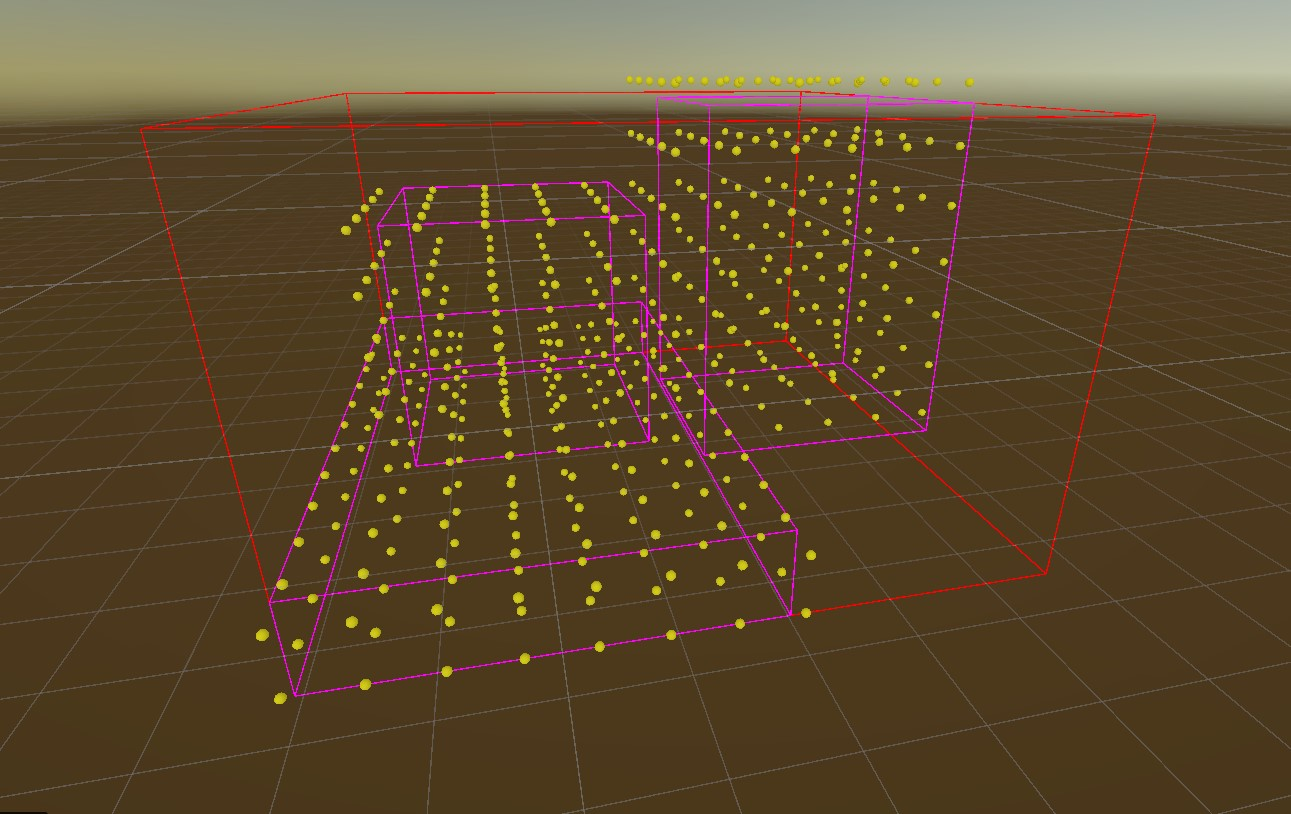
\includegraphics[scale=0.43]{Graphics/Grid_Example.jpg}
	\caption{A 3D Scene showing the placement of Evaluation Points (shown in yellow) inside the user defined bounds (shown in pink), contained within the calculated volume (shown in red).}
	\label{fig:grid}
\end{figure}

After placing the EP, we use each point to calculate the data needed for the feature vectors. The aim of the LPNN model is to give an importance value to each of those EP that it is given. Therefore, it is vital that it understands what defines a significant point via the features that it is trained on. Our knowledge dictates that an important location for a light probe is one that has great variance in illumination. Therefore, we include light-, RGB- and normal-variance as features for each point. Light-Variance dictates how much the light intensity changes around a point. RGB-Variance is similar, since it shows the change in Red, Green, and Blue light around each point, each channel being independent from the others. Normal-Variance is a value that makes locations like corners distinct from empty areas or from locations near a wall. Similarly, we also calculate Occlusion-Factor, a feature that gives each point a value depending on how empty or cluttered the area around it is. Normal-Variance together with Occlusion-Factor inform the model of areas that are enclosed or close to complex geometry. This makes the model able to distinguish these locations, even when all other values are identical, making it able to give different importance values to those distinct locations.

Along with the features mentioned above, we additionally include a vector that contains the spherical-harmonic values for a small amount of distinct directions around each point. The implementations of each feature collection method are shown in \ref{alg:feat_sh}, \ref{alg:feat_lv}, \ref{alg:feat_rgbv}, \ref{alg:feat_nv}, and \ref{alg:feat_of}.


\begin{algorithm}
	\caption{Feature Extraction: Spherical Harmonics around a point}
	\label{alg:feat_sh}
	\begin{algorithmic}[1]
		\Require $EP \neq \emptyset$
		\State $values = \emptyset$
		\ForAll{$points \in EP$}
			\State $value \gets evaluateSH(point)$
			\State $values \gets values + value$ \Comment Append SH to the list
		\EndFor
		\State \Return $values$
	\end{algorithmic}
\end{algorithm}

\begin{algorithm}
	\caption{Feature Extraction: Light Variance around a point}
	\label{alg:feat_lv}
	\begin{algorithmic}[1]
		\Require $EP \neq \emptyset$
		\Require $samples \geq 1$ \Comment The amount of directions
		\State $radius \gets 1$ \Comment How far around the point to check
		\ForAll{$points \in EP$}
			\State $luminances = \emptyset$
			\For{$n = 1,\dots,samples$}
				\State $direction \gets$ random point on sphere with $radius$
				\State $sh \gets evaluateSH(direction)$
				\State $luminance \gets sh.R * 0.2126 + sh.G * 0.7152 + sh.B * 0.0722$ \Comment From RGB to luminance value
				\label{alg:feat_lv:7}
				\State $luminances \gets luminances + luminance$ \Comment Add luminance to the list
			\EndFor
			\State $mean \gets mean(luminances)$ \Comment Get the mean value of the luminances
			\State $variance \gets (luminances - mean)^2 \div samples$ \Comment Get the total variance of luminances
		\EndFor
		\State \Return $variance$ per point
	\end{algorithmic}
\end{algorithm}

In line \algref{alg:feat_lv}{alg:feat_lv:7}, to convert from RGB channel values to perceived light intensity of the pixel, also known as luminance, we use the formula shown in \cite{Luminance2015}, under section 3 item 3.2. This formula is used to calculate how bright a pixel in regards to the RGB channel values it currently shows.

Similarly, we collect the RGB-Variance independently for each channel. The formula is similar to Light-Variance, with the exception of line \algref{alg:feat_lv}{alg:feat_lv:7}, since it is not applicable. We need each channel RGB value to be unaffected by any conversion. This is seen in algorithm \ref{alg:feat_rgbv}.

\begin{algorithm}
	\caption{Feature Extraction: RGB Variance around a point}
	\label{alg:feat_rgbv}
	\begin{algorithmic}[1]
		\Require $EP \neq \emptyset$
		\Require $samples \geq 1$ \Comment The amount of directions
		\State $radius \gets 10$ \Comment How far around the point to check
		\ForAll{$points \in EP$}
			\State $count \gets 0$
			\For{$n = 1,\dots,samples$}
				\State $direction \gets$ random point on sphere with $radius$
				\State $sh \gets evaluateSH(direction)$
			\EndFor
			\State $meanRGB \gets mean(sh.RGB)$
			\State $RGBvariance \gets (sh.RGB - meanRGB)^2 \div samples$
		\EndFor
		\State \Return ${RGBvariance.R, RGBvariance.G, RGBvariance.B}$ per point
	\end{algorithmic}
\end{algorithm}

\begin{algorithm}
	\caption{Feature Extraction: Normal Variance around a point}
	\label{alg:feat_nv}
	\begin{algorithmic}[1]
		\Require $EP \neq \emptyset$
		\Require $samples \geq 1$ \Comment The amount of directions
		\State $radius \gets 1$ \Comment How far around the point to check
		\ForAll{$points \in EP$}
			\State $normals = \emptyset$
			\For{$n = 1,\dots,samples$}
				\State $direction \gets$ random point on sphere with $radius$
				\State $hit \gets castRay(direction)$
				\If{$hit == True$}
					\State $normals \gets normals + hit.normal$
				\EndIf
			\EndFor
			\State $mean \gets mean(normals)$ \Comment Get the mean direction of the normals
			\State $variance \gets (1- dot(normals, mean)) \div samples$
			\label{alg:feat_nv:12}
			\Comment Get the total variance of normals
		\EndFor
		\State \Return $variance$ per point
	\end{algorithmic}
\end{algorithm}

In line \algref{alg:feat_nv}{alg:feat_nv:12}, we want the higher values to define the areas with more complex geometry. The dot product of vectors is a value between 0 and 1, therefore we subtract the dot product from 1, to invert the range of the variance.

\begin{algorithm}
	\caption{Feature Extraction: Occlusion Factor around a point}
	\label{alg:feat_of}
	\begin{algorithmic}[1]
		\Require $EP \neq \emptyset$
		\Require $samples \geq 1$ \Comment The amount of directions
		\State $radius \gets 10$ \Comment How far around the point to check
		\ForAll{$points \in EP$}
			\State $count \gets 0$
			\For{$n = 1,\dots,samples$}
				\State $direction \gets$ random point on sphere with $radius$
				\State $hit \gets castRay(direction)$
				\If{$hit == True$}
					\State $count \gets count + 1$
				\EndIf
			\EndFor
			\State $factor \gets count \div samples$
			\Comment Percentage of hits versus misses.
		\EndFor
		\State \Return $factor$ per point
	\end{algorithmic}
\end{algorithm}

Similarly to algorithm \ref{alg:feat_nv}, algorithm \ref{alg:feat_of} casts rays around each point, the amount determined by the $samples$ variable, for a certain distance, determined by the $radius$ variable. Each time a ray collides with any object, we increment a variable. At the end, we calculate the percentage of rays that collided to the total rays cast, and we return the result for each point. Higher values describe points that are surrounded to geometry in close proximity.

After collecting all the features, we compact them into a feature vector per-EP, and save them into a file for use during training, or directly for light probe placement, as we will see shortly. As shown in section \ref{sec:LPNN_UI}, it is also possible to collect feature vectors from multiple scenes at different times, as well as labels, to make the model more accurate by providing more input data. 

\section{Label Collection}

The supervised-learning approach we decided on for this thesis requires that the model also receives labels as an input. Labels are values for each of the input feature vectors that describe the correct output for that feature vector. It is therefore vital to collect labels for each EP that we have also collected features for. For this purpose, we use LumiProbes \parencite{Vardis2021} to collect labels by returning a True or False value, depending on if the cell of each Evaluation Point contains a probe placed by LumiProbes. The use of LumiProbes as the ground-truth was arbitrary. The system is constructed in a way that allows any method of ground-truth light probe placement to be used for label extraction, even manual placement. In algorithm \ref{alg:labels} we check every EP with every light probe in the ground-truth list and set the label to True if there exists a light probe around a \textit{cellsize} radius of that Evaluation Point.

\begin{algorithm}
	\caption{Label Extraction per-EP}
	\label{alg:labels}
	\begin{algorithmic}[1]
		\Require $EP \neq \emptyset$
		\Require $cellsize > 0$
		\ForAll{$points \in EP$}
			\ForAll{$probes \in groundTruth$}
				\If{$probe \in cellsize$ around $point$}
				\Comment If the probe is within the cell of each point...
					\State $label \gets True$
				\Else
					\State $label \gets False$
				\EndIf
			\EndFor
		\EndFor
		\State \Return $labels$ per point
	\end{algorithmic}
\end{algorithm}

The nature of this label extraction method beckons for the ground-truth light probe placement to be close to the optimal placement, determined by the user's intuition, experience, and demands for the specific scene.

After collecting the labels into a list, they are saved into a file on the hard disk for use in training of the model, as seen in section \ref{sec:model_training}. As mentioned previously, it is possible to collect labels from multiple scenes, creating a bigger dataset for the model to train on.

\section{Model Training}
\label{sec:model_training}

The model basis for LPNN, as described in section \ref{sec:background:pointnet}, was a PointNet architecture \parencite{PointNet2017}. We followed the style loosely, mainly focusing on making a model that is able to predict importance scores per-point, and able to handle an arbitrary amount of input points without retraining. 

\subsection{Data Preparation}
The feature vectors that were created from the previous steps are read from the files stored on the hard disk. For the labels, we convert each True or False line into numerical 1 or 0, respectively. Then, a Numpy array is created, containing all the values in order of appearance.
For the feature vectors, a similar method is used. Additional logic is needed since there are multiple values per line, but the features are finally converted into an array of arrays. Each sub-array contains the values per-point, in order of appearance.

\subsection{Model Architecture \& Training}

The architecture is as follows; First, three Convolution1D layers followed by three Batch Normalization layers expand the input from a feature vector of length 30 to 256. Each of these 6 layers are used one after the other, first a Convolution1D with dimensions 64x30x1x1 and a ReLu activation, followed by a Batch Normalization layer, then the next Convolution1D layer with dimensions 128x64x1x1 with the same activation function, etc. Then, in order for the model to have some knowledge of the global context, we use a Global Max Pooling 1D layer and a Global Average Pooling Layer 1D, concatenated together with each per point local context, resulting in a 512 dimensional feature layer. 

In order to avoid averaging all neurons together for each point, we tile the global context, using a custom tiling function, making each neuron have knowledge of only the surrounding points, instead of every point in the scene. This ensures that each point's significance will only be affected by the surrounding lighting data of itself and the nearby points. However, this method also ensures that each point still has some knowledge of information beyond the tile that it was trained on, since the global pooling is done before the tiling. Therefore, each tile is only a piece of the total, but contains the information that was affected by the global pooling layers. This makes each point not completely agnostic to the global environment beyond the tile it was trained on, but it also makes the point more sensitive to surrounding data within each tile.

Finally, another Convolution1D and Dropout sequence is used to reduce the high-dimensional hidden layers into a single importance score $i \in [0,1]$. The Dropout layers are important to reduce learning error rates by randomly deactivating a small set of neurons and their connections during the training process. The probability for drop-out is set to 0.3, meaning 30\%. This sequence of layers are then directed into another Convolution1D layer with Sigmoid activation function, and trained for 50 epochs.The model is then compiled and saved in an .onnx file for import back into the Unity engine.

\begin{figure}[h]
	\centering
	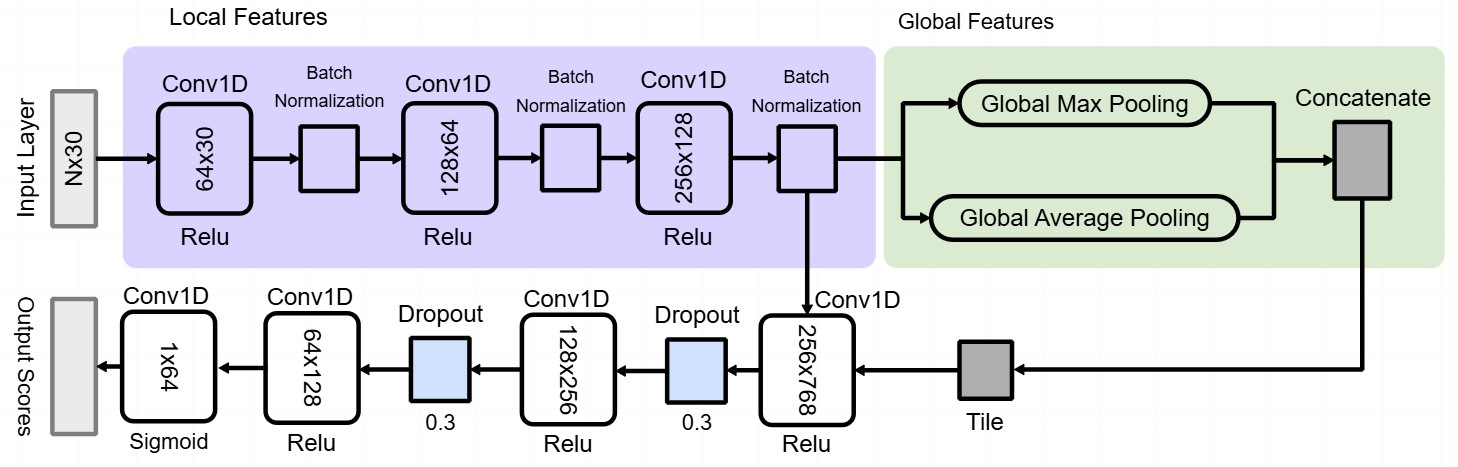
\includegraphics[scale=0.392]{Graphics/LPNN.jpg}
	\caption{Neural Network architecture of our LPNN model.}
	\label{fig:LPNN_arch}
\end{figure}

\section{Light Probe Prediction}
In order to use the model to infer importance scores for the EP, we need to import it to Unity. For this purpose, we use Sentis. After model import, it can be used for our goals. First, since the model is agnostic to each scene and each EP layout, we need to provide it with the feature vector list, containing the feature vector for each EP. This process is the same as in \ref{sec:feature_collection}, therefore it is not described again. The only exception is that the list is not saved into a file at the end of the process, since it will be used directly inside Unity, therefore we only need the variable that contains the list object inside the code implementation.

First, it is necessary to convert the feature vectors into the same data format that was used when the model was trained using Python and TensorFlow. Providing any other format will result in the program not executing correctly, causing an error message or even a crash. This is because Sentis is able to execute model inference workloads on the GPU for parallelism and therefore faster execution. This is optional, since Sentis has a fallback feature. If no capable GPU is detected on the system, it uses the system's CPU instead. We have set Sentis to prefer using GPU compute for faster execution even with larger datasets, but the CPU fallback makes sure no additional logic is needed in cases where the system used does not contain a GPU. 

After converting the vectors into the correct format, the compute device that was chosen is then sent the data and requested to infer using the model that we trained. This is done asynchronously, meaning that the execution of the code is not halted while the device is processing. It is therefore possible to request the inferred values back at a later time, but that is not necessary for our use-case. We save the inferred values to a file on the hard disk, meaning we can perform calculations on the values without affecting the original list, as we will see shortly, and remain able to read the original values without needing to re-infer using the model.

After inferring, the Light probe group can now be populated according to the inferred importance scores. For that purpose, as seen in algorithm \ref{alg:lp_place}, it is necessary to pre-process all the values for better handling. It is not unlikely that the scores given by the model are very concentrated to some value, sometimes clusters forming in the data, making the use of the threshold system delicate. To fix this, we remap the range of the values from the minimum and maximum value to 0 and 1. This results in the values covering the entirety of the output range 0-1, instead of potentially only parts of it, spreading out any clustering of values.

\begin{algorithm}
	\caption{Inferred Scores Range Remapping}
	\label{alg:lp_place}
	\begin{algorithmic}[1]
		\Require $inferredValues \neq \emptyset$
		\Comment The inferred value list from the model.
		\State $min \gets \inf$
		\Comment Positive Infinity
		\State $max \gets -\inf$
		\Comment Negative Infinity
		\ForAll{$value \in inferredValues$}
			\If{$value < min$}
				\State $min \gets value$
			\ElsIf{$value > max$}
				\State $max \gets value$
			\EndIf
		\EndFor
		\ForAll{$value \in inferredValues$}
			\State $value \gets (value - min) / (max - min)$
			\Comment After calculating minimum and maximum, we remap the values
			\label{alg:lp_place:11}
		\EndFor
		\State \Return $values$ list
	\end{algorithmic}
\end{algorithm}

The complete function for remapping a value $x$ from a \([min1, max1]\) range to another \([min2, max2]\) range is as follows:

\[ result = min2 + (max2 - min2) * ((x - min1)/(max1 - min1)) \]

For our purposes, the ranges are \([min, max]\) and \([0, 1]\). Therefore, the function can be simplified to the one seen in \algref{alg:lp_place}{alg:lp_place:11}.

With the values remapped, the threshold system can be used without delicate control. We decided on a percentile threshold system, meaning that the user can decide what percentage of the total amount of light probes they want to be placed, with the most important ones appearing first. The algorithm for this is simple, as seen in \ref{alg:lp_thres}. First, we duplicate the list, leaving the original unaffected, which the duplicate is then sorted in a descending order. Then, from the ordered list, the top percentage of the values is kept, depending on the threshold value that is currently set by the user.

\begin{algorithm}
	\caption{Thresholded Placement of Light Probes}
	\label{alg:lp_thres}
	\begin{algorithmic}[1]
		\Require $inferredValues \neq \emptyset$
		\Require $threshold \in [0, 1]$
		\Comment The threshold given by the user
		\State $percentage \gets ((1-threshold) * inferredValues.count)$
		\Comment Calculate the amount requested by the threshold value, from the total
		\label{alg:lp_thres:1}
		\State $duplicate \gets inferredValues.copy$
		\State $duplicate \gets sort(duplicate).copyAmount(percentage)$
		\Comment Sort the duplicate list and keep only the desired amount
		\ForAll{$value \in duplicate$}
			\State $positions \gets positions + inferredValues.indexOf(value)$
			\Comment append the EP to the desired positions list
		\EndFor
		\State $LightProbeGroup.positions = positions$
		\State \Return $Light Probe Group$
	\end{algorithmic}
\end{algorithm}

In line \algref{alg:lp_thres}{alg:lp_thres:1}, we invert the threshold, since, as mentioned before, we want the higher-importance values to appear first. This means that with a 90\% threshold, the top 10\% light probes with the highest importance score should be placed, while the remaining 90\% with lower significance should be ignored. 

Finally, we set the positions of the Light Probe Group Unity object to be the ones that are within the threshold that we calculated, seen as the $positions$ variable in the algorithm mentioned. As we will see in section \ref{sec:LPNN_UI}, the light probes are now placed in the scene and visible to the user, completing the execution of the tool.

\section{LPNN inside Unity Editor}
\label{sec:LPNN_UI}
